\begin{frame}[ctb!]
\frametitle{Specific Temperature Change Calculations}
\footnotesize{A reference data set of temperature change curves was calculated. 
Repeated runs of a detailed model over the range of values in Table 
\ref{tab:thermal_cases} determined Specific Temperature Change (STC) values over a range of thermal 
heat limit radii, $r_{lim}$, thermal diffusivity values, $\alpha_{th}$,
thermal conductivity values, $K_{th}$ and waste package spacings, $S$.

\begin{table}[ht!]
\centering
\footnotesize{
\begin{tabular}{|l|l|l|r|}
\multicolumn{4}{c}{\textbf{Thermal Cases}}\\
\hline
\textbf{Parameter} & \textbf{Symbol} & \textbf{Units} & \textbf{Value Range} \\
\hline
Diffusivity & $\alpha_{th}$ & $[m^2\cdot s^{-1}]$ & $1.0\times10^{-7}-3.0\times10^{-6}$\\
\hline
Conductivity & $K_{th}$     & $[W\cdot m^{-1} \cdot K^{-1}]$ & $0.1 - 4.5$ \\
\hline
Spacing & $S$ & $[m]$ & 2, 5, 10, 15, 20, 25, 50 \\
\hline
Radius & $r_{lim}$ & $[m]$ & 0.1, 0.25, 0.5, 1, 2, 5 \\
\hline
Isotope & $i$ & $[-]$ & $^{241,243}Am,$  \\
        & & & $^{242,243,244,245,246}Cm,$  \\
        & & & $^{238,240,241,242}Pu$  \\
        & & & $^{134,135,137}Cs$  \\
        & & & $^{90}Sr$  \\
\hline
\end{tabular}
\caption{A thermal reference dataset of \gls{STC} values as a function of each of these parameters was generated by repeated parameterized runs of the LLNL 
MathCAD model\cite{greenberg_application_2012, greenberg_investigations_2012}.}
\label{tab:thermal_cases}
}
\end{table}


}
\end{frame}


\begin{frame}[ctb!]
\frametitle{LLNL UFD MathCAD Model}
\footnotesize{
The analytic model used to populate the reference dataset was created at 
LLNL for the UFD campaign \cite{hardin_generic_2011, 
greenberg_investigations_2012, greenberg_application_2012}. It employs an 
analytic model from Carslaw and Jaeger and is \textbf{implemented in MathCAD}
\cite{carslaw_conduction_1959, ptc_mathcad_2010}.  The integral solver in the 
MathCAD toolset is the primary calculation engine for the analytic MathCAD 
thermal model, which relies on superposition of point, finite-line, and line 
source integral solutions.  
}
\end{frame}
% LLNL
\subsection{Analytical Model Background}
\begin{frame}[ctb!]
\frametitle{Analytical Model : Background}
The analytical  model
\begin{itemize} 
  \item was created at LLNL (H. Greenberg, J. Blink, et. al) \cite{hardin_generic_2011, sutton_investigations_2011, 
greenberg_application_2012}
  \item employs an analytic model from Carslaw and Jaeger \cite{carslaw_conduction_1959} 
  \item is implemented in MathCAD \cite{ptc_mathcad_2010}
  \item seeks to inform heat limited waste capacity calculations for 
    \begin{itemize}
      \item arbitrary geology 
      \item arbitrary waste package loading densities
      \item arbitrary homogeneous decay heat source
    \end{itemize}
\end{itemize}
\end{frame}

\begin{frame}
  \frametitle{Analytical Model : Geometry}
  \begin{figure}[h!]
    \begin{center}
      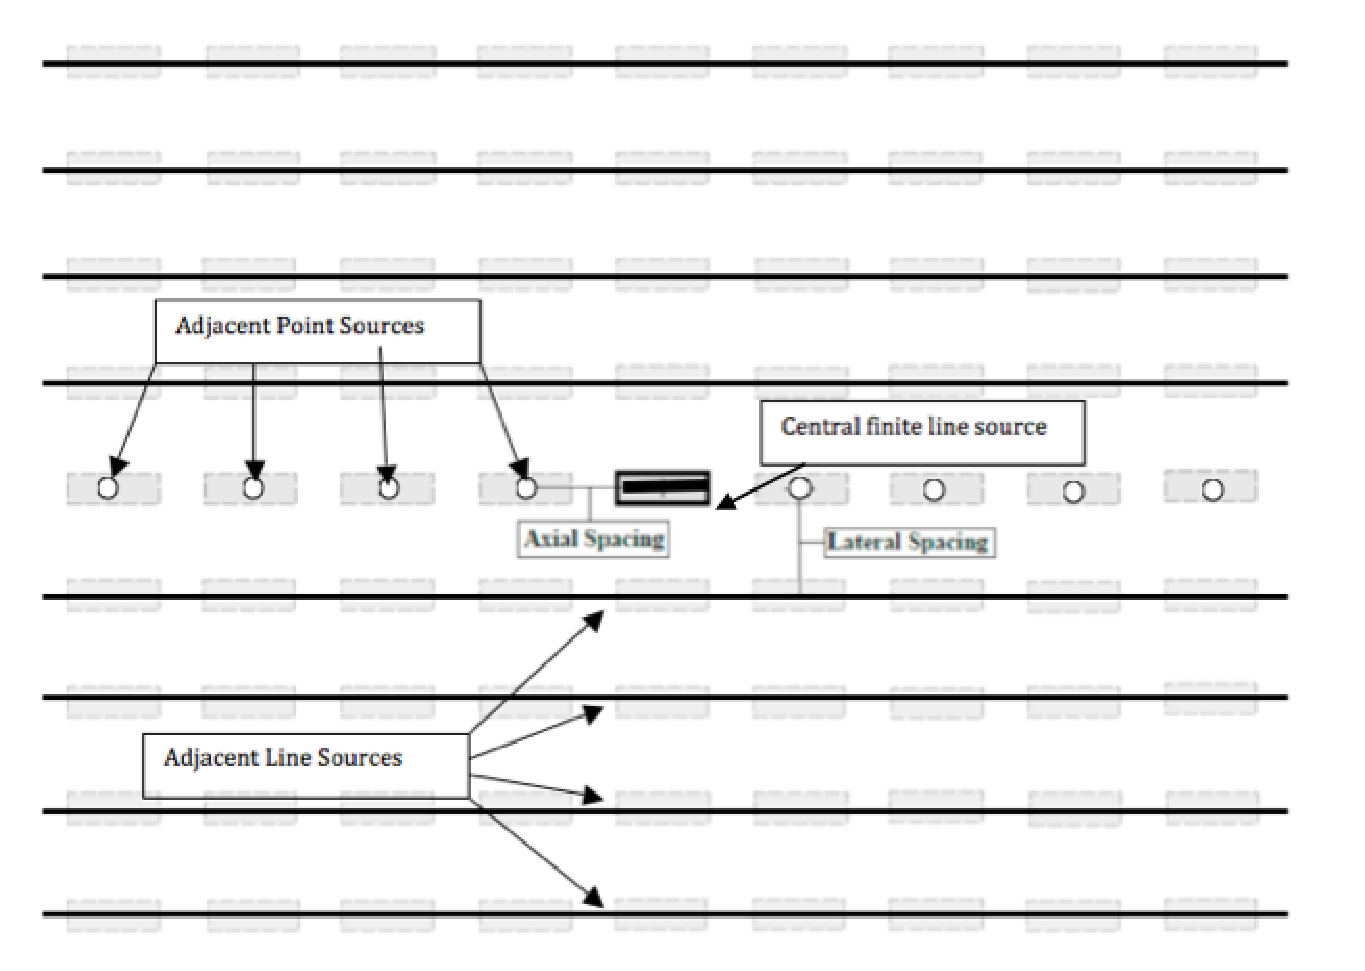
\includegraphics[width=0.7\textwidth]{./images/llnlConcept.eps}
    \caption{Vertical, horizontal, alcove, and borehole emplacement layouts can 
    be represented by a line of point sources and adjacent line sources 
    \cite{sutton_investigations_2011}.}
    \label{fig:llnl}
    \end{center}
  \end{figure}
\end{frame}

\begin{frame}
  \frametitle{Analytical Model : Calculation Method}
    LLNL's model is a MathCAD solution of the transient homogeneous 
    conduction equation,
    \begin{align}
      \nabla^2T  = \frac{1}{\alpha}\frac{\partial T}{\partial t},
      \label{condGl}
    \end{align}
    in which superimposed point and line source solutions approximate the repository 
    layout.
\end{frame}

\begin{frame}[ctb!]
\frametitle{Analytical Model : Calculation Method}
The model consists of two conceptual regions, an external region representing 
the host rock and an internal region representing the waste form, package, and 
buffer Engineered Barrier System within the disposal tunnel wall.   
\begin{itemize}
  \item Since the thermal mass of the EBS is small in comparison to the thermal 
    mass of the host rock, the internal region may be treated as quasi-steady 
    state.
  \item The transient state of the temperature at the calculation radius is 
    found with a convolution of the transient external solution with the steady 
    state internal solution.
  \item The internal and external regions are \textbf{approximated} to be a 
    single homogeneous medium.
  \item The process is then iterated with a one year resolution in order to 
    arrive at a temperature evolution over the lifetime of the repository. 
\end{itemize}
\end{frame}


\begin{frame}[ctb!]
\frametitle{Analytical Model : Calculation Method}
\begin{minipage}{0.3\textwidth}
\begin{figure}[h!]
  \begin{center}
    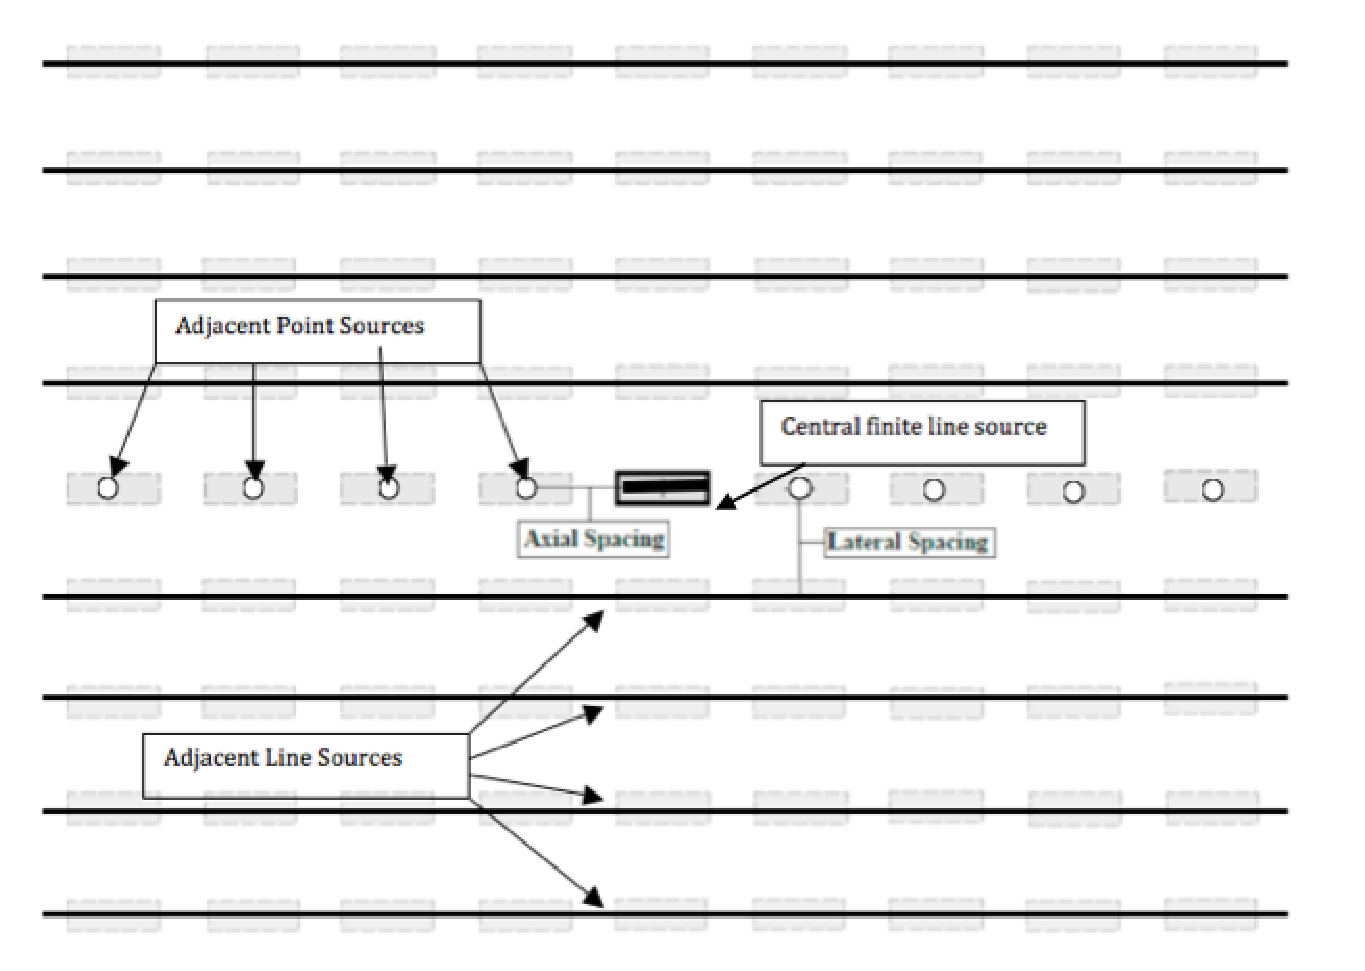
\includegraphics[width=\textwidth]{./images/llnlConcept.eps}
  \end{center}
  \caption{The central package is represented by a finite line source
  \cite{sutton_investigations_2011}.}
  \label{fig:llnl}
\end{figure}
\end{minipage}
\hspace{0.01mm}
\begin{minipage}{0.6\textwidth}
The geometric layout of the analytic LLNL model in Figure \ref{fig:llnl} 
shows  that the central package is represented by the finite line solution
\footnotesize{
\begin{align}
  T_{line}&(t,x,y,z) = \nonumber\\
  &\frac{1}{8\pi K_{th}} 
  \bigintsss_0^t\!\frac{q_L(t')}{t-t'}e^{ \frac{-\left(x^2 + z^2\right)}{4\alpha 
  (t-t')} }\nonumber\\ &\cdot\left[ \erf{\left[ \frac{1}{2} \frac{\left( y + 
  \frac{L}{2} \right)}{\sqrt{\alpha(t-t')}}  \right]} - \erf{\left[ \frac{1}{2} 
  \frac{\left( y - \frac{L}{2} \right)}{\sqrt{\alpha(t-t')}}  \right]} 
  \right]\,\mathrm{dt'}.
  \label{line}
\end{align}
}
\end{minipage}
\end{frame}

\begin{frame}[ctb!]
\frametitle{Analytical Model : Calculation Method}
\begin{minipage}{0.3\textwidth}
\begin{figure}[h!]
  \begin{center}
    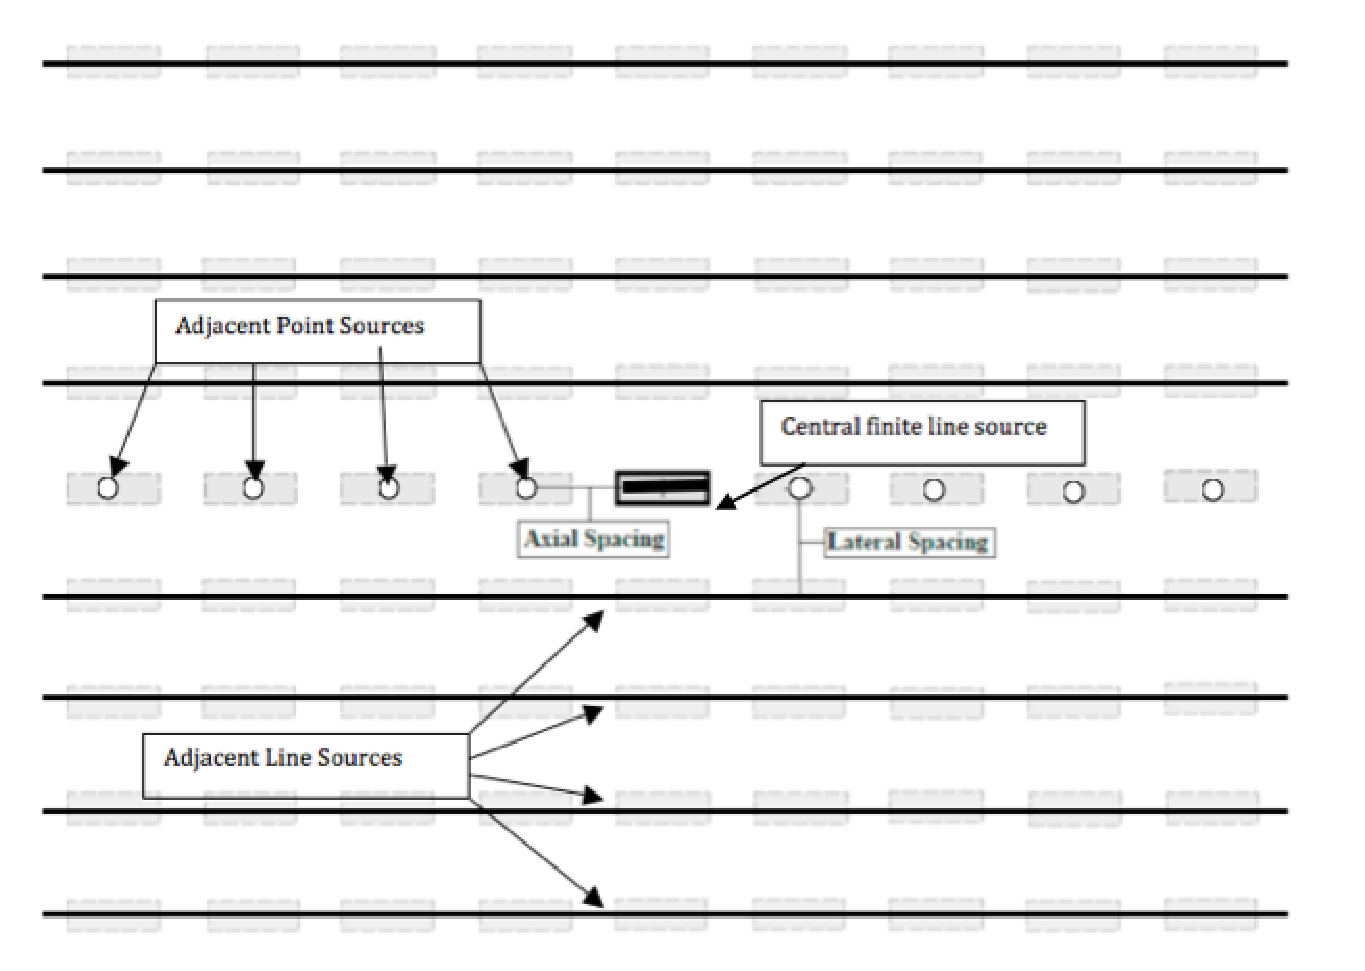
\includegraphics[width=\textwidth]{./images/llnlConcept.eps}
  \end{center}
  \caption{Adjacent packages are represented as point sources
  \cite{sutton_investigations_2011}.}
  \label{fig:llnl}
\end{figure}
\end{minipage}
\hspace{0.1mm}
\begin{minipage}{0.6\textwidth}
 Adjacent packages within the central tunnel are represented by the point source 
 solution,
 \footnotesize{
  \begin{align}
    T_{point}(t,r) &= \frac{1}{8K_{th}\sqrt{\alpha}\pi^{\frac{3}{2}}}\nonumber\\
     &\bigintsss_0^{t}\!\frac{q(t')}{(t-t')^{\frac{3}{2}}}e^{\frac{-r^2}{4\alpha(t-t')}}\,\mathrm{dt'}.
    \label{point}
  \end{align}
  }
  \end{minipage}
\end{frame}


\begin{frame}[ctb!]
\frametitle{Analytical Model : Calculation Method}
\begin{minipage}{0.3\textwidth}
\begin{figure}[h!]
  \begin{center}
    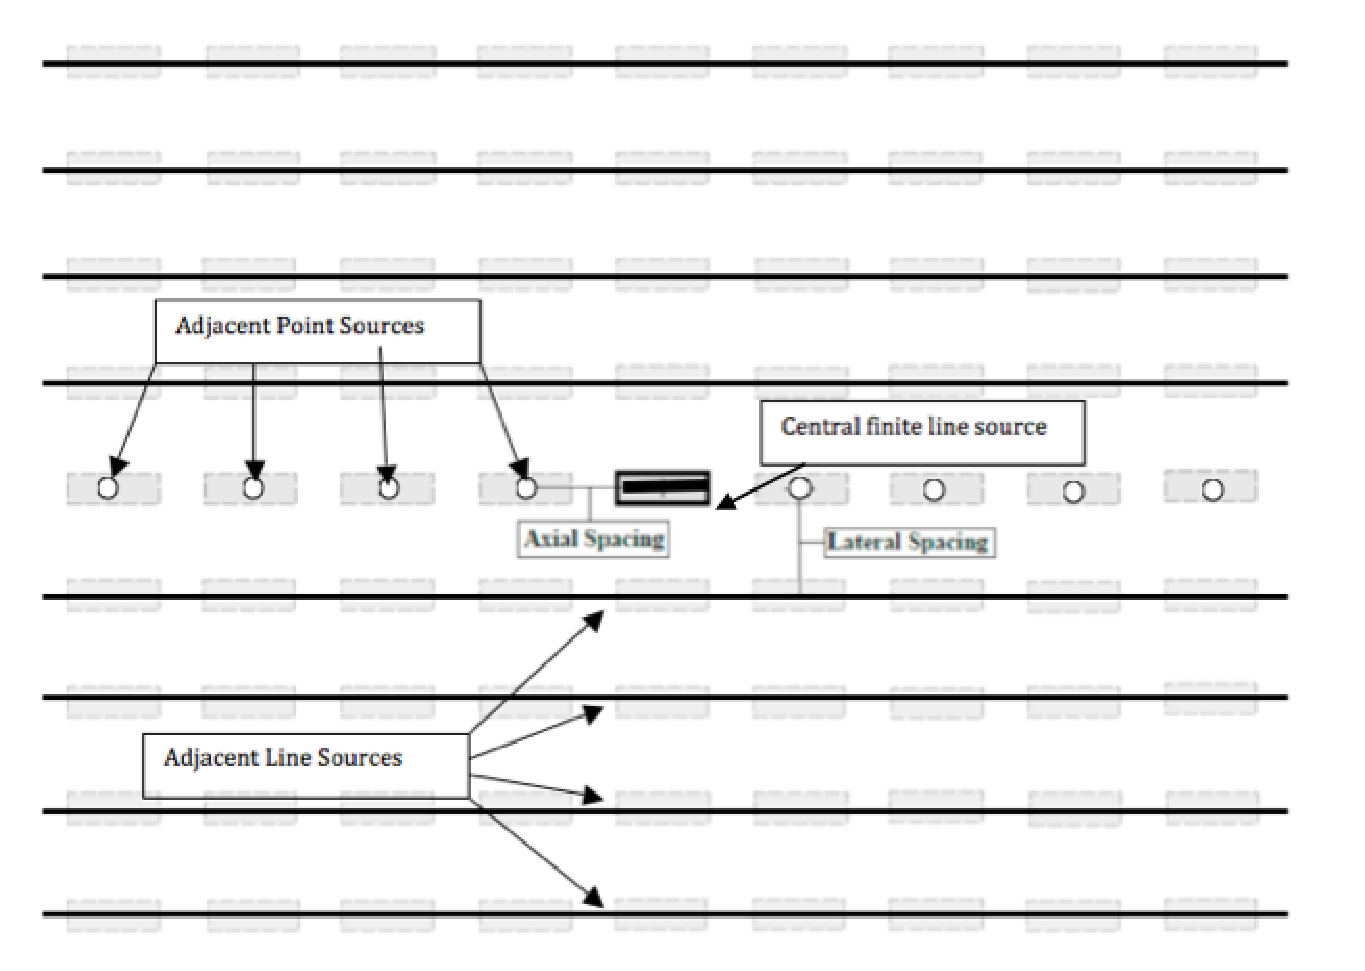
\includegraphics[width=\textwidth]{./images/llnlConcept.eps}
  \end{center}
  \caption{The non-central disposal tunnels are represented as infinite line sources
  \cite{sutton_investigations_2011}.}
  \label{fig:llnl}
\end{figure}
\end{minipage}
\hspace{0.1mm}
\begin{minipage}{0.6\textwidth}
Adjacent disposal tunnels are represented by the infinite line source solution,
\footnotesize{
\begin{align}
  T_{\infty line}(t,x,z) &= \frac{1}{4\pi K_{th}} 
  \bigintsss_0^t\frac{q_L(t')}{t-t'}e^{ \frac{-\left(x^2 + z^2\right)}{4\alpha 
  (t-t')} }
  \label{infline}
  \intertext{in infinite homogeneous media, where}
  \alpha &= ~~\mbox{thermal diffusivity } [m^2\cdot s^{-1}]\nonumber\\
  q(t) &= ~~\mbox{point heat source} [W]\nonumber\\
  \intertext{and}
  q_L(t) &= ~~\mbox{linear heat source} [W\cdot m^{-1}]\nonumber
\end{align}
}
Superimposed point and line source solutions allow for a notion of the 
repository layout to be modeled in the host rock.
\end{minipage}
\end{frame}





\begin{frame}[ctb!]
\frametitle{Scaling Demonstration}
\footnotesize{

\begin{figure}[h!]
\begin{center}
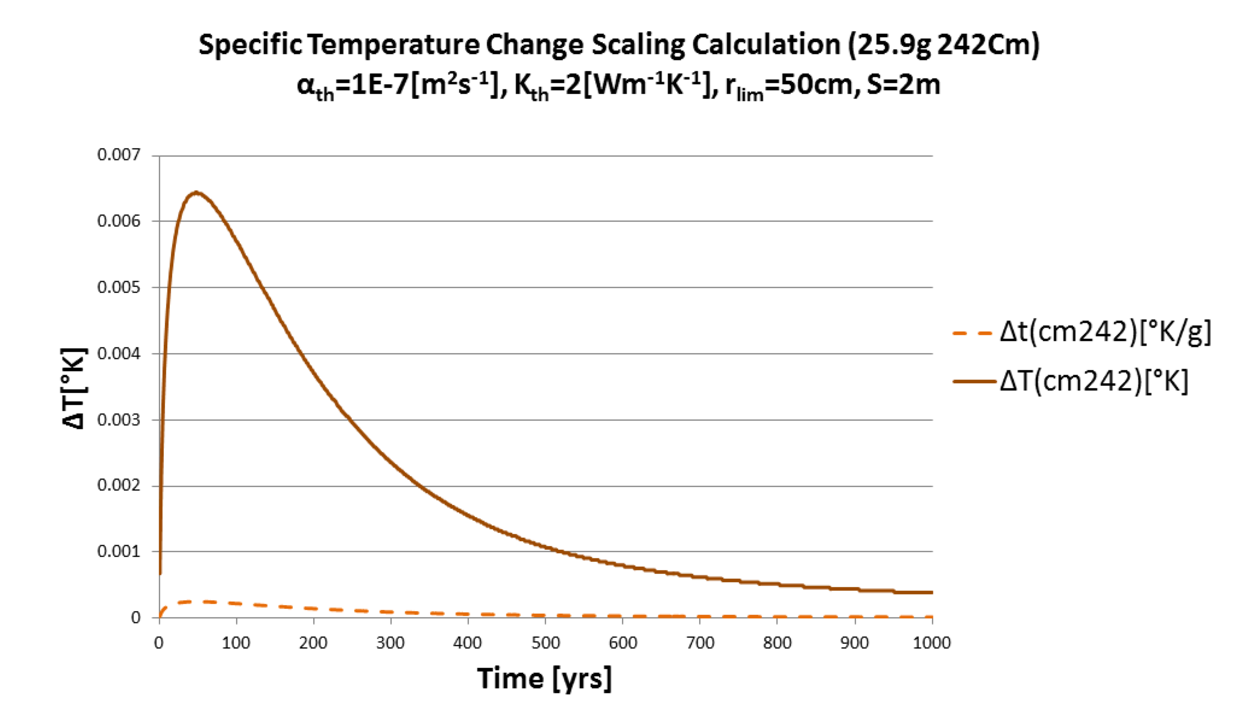
\includegraphics[width=\linewidth]{./images/CmScaling.eps}
\end{center}
\caption{As a demonstration of the calculation procedure, the temperature change 
  curve for one initial gram of $^{242}Cm$ and is scaled to represent $25.9g$, 
  approximately the $^{242}Cm$ inventory per MTHM in 51GWd burnup UOX PWR fuel. }
\label{fig:CmScaling}
\end{figure}
}
\end{frame}

\begin{frame}
\frametitle{Superposition Concept}
\footnotesize{

The supporting database was limited to some primary heat contributing isotopes 
present in traditional spent nuclear fuel, $H$, 
such that the superposition in equation \eqref{superposition} becomes 
\begin{align}
\Delta T (r_{lim},S,K_{th},\alpha_{th})&\sim \sum_{i\in H} m_i \Delta t_i(r_{lim},S,K_{th},\alpha_{th})
\label{superposition_approx}
\intertext{where}
H &= \mbox{ set of high heat isotopes }[-]\nonumber\\
S &= \mbox{ uniform waste package spacing } [m]\nonumber\\
K_{th} &= \mbox{ thermal conductivity } [W\cdot m^{-1}\cdot K^{-1}]\nonumber\\
\alpha_{th} &= \mbox{ thermal diffusivity } [m^2\cdot s^{-1}]\nonumber\\
\end{align}
}
\end{frame}


\begin{frame}
\frametitle{Superposition Demonstration}
\footnotesize{

\begin{figure}[ht!]
\begin{center}
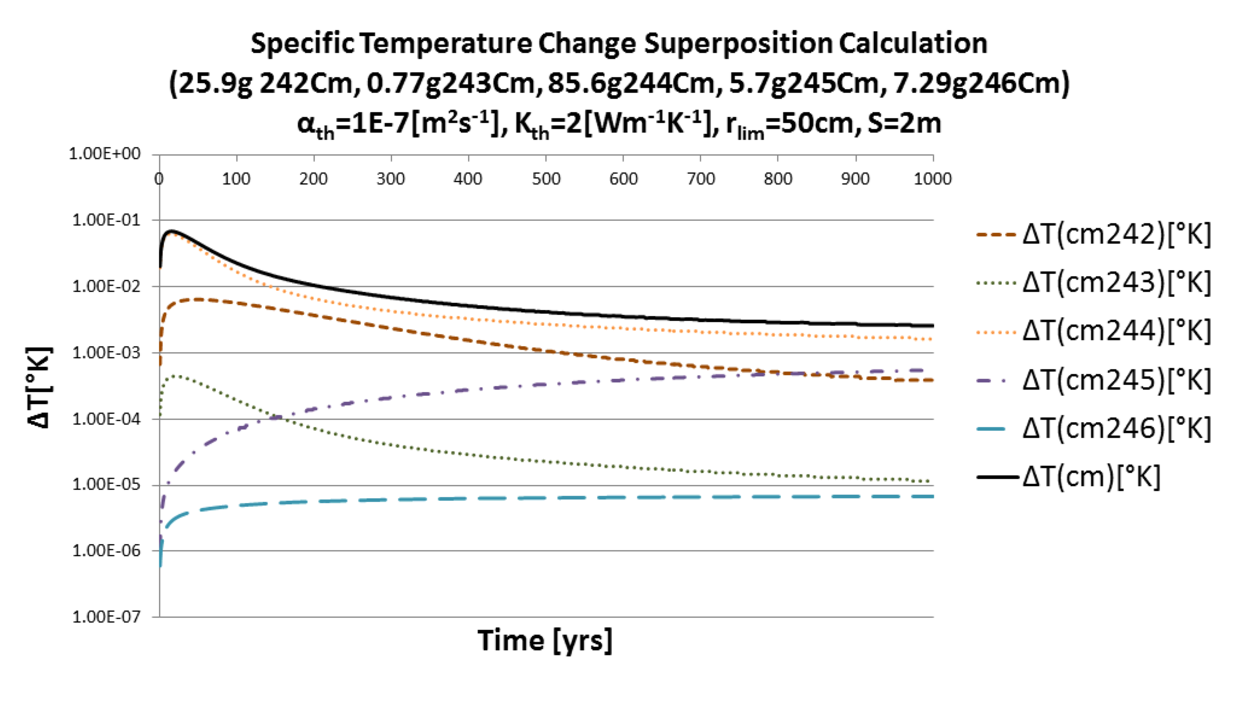
\includegraphics[width=\columnwidth]{./images/CmSuperposition.eps}
\end{center}
\caption{As a demonstration of the calculation procedure, scaled temperature change 
  curves for five curium isotopes are superimposed to achieve a total temperature 
change (note log scale).}
\label{fig:CmSuperposition}
\end{figure}

}
\end{frame}


